\documentclass[tikz,border=2pt]{standalone}
\usepackage{amsmath}
\usepackage{tikz}

\begin{document}
% A ⊆ B: every element of A is also an element of B, so A sits inside B.
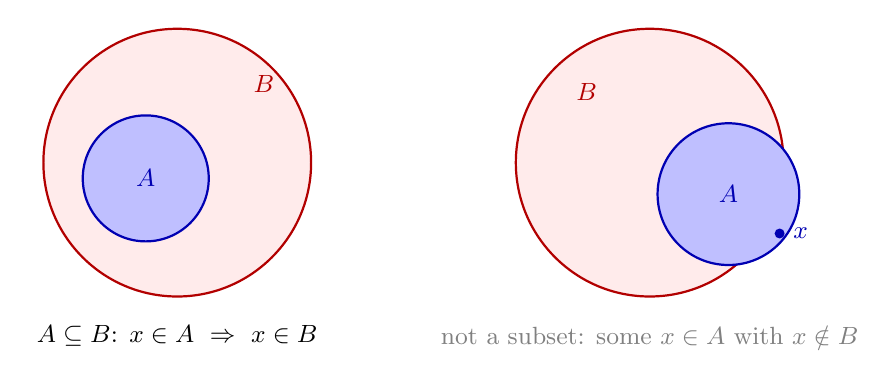
\begin{tikzpicture}[every node/.style={font=\small}]
	\draw[thick, red!70!black, fill=red!8] (0,0) circle (1.7);
	\draw[thick, blue!70!black, fill=blue!25] (-0.4,-0.2) circle (0.8);
	\node[blue!70!black] at (-0.4,-0.2) {$A$};
	\node[red!70!black] at (1.1,1.0) {$B$};
	\node at (0,-2.2) {$A\subseteq B$: $x\in A\ \Rightarrow\ x\in B$};
	\begin{scope}[xshift=6cm]
		\draw[thick, red!70!black, fill=red!8] (0,0) circle (1.7);
		\draw[thick, blue!70!black, fill=blue!25] (1.0,-0.4) circle (0.9);
		\node[blue!70!black] at (1.0,-0.4) {$A$};
		\node[red!70!black] at (-0.8,0.9) {$B$};
		\fill[blue!70!black] (1.65,-0.9) circle (1.8pt);
		\node[blue!70!black, right] at (1.7,-0.9) {$x$};
		\node[gray] at (0,-2.2) {not a subset: some $x\in A$ with $x\notin B$};
	\end{scope}
\end{tikzpicture}
\end{document}
